% !TEX root = ../main.tex

\chapter{Technology}
\label{ch:technology}

\startcontents[chapters]

\vfill

\begin{alltt}\sffamily
Ten thousand soldiers with me I will take,
only thus much I give your Grace to know,
the tenth of August last this dreadful lord,
I'll give thee this neck.

He did so set his teeth and tear it,
the circumstance I'll tell you more at large,
or ten times happier be it ten for one,
if he will touch the estimate.

And tell me he that knows,
a thousand knees ten thousand years together,
stand on the dying neck.

Towards school with heavy looks,
and thus do we of wisdom and of reach,
be an arch.
\end{alltt}

\newpage
\begin{figure}[!htbp]
\centering
  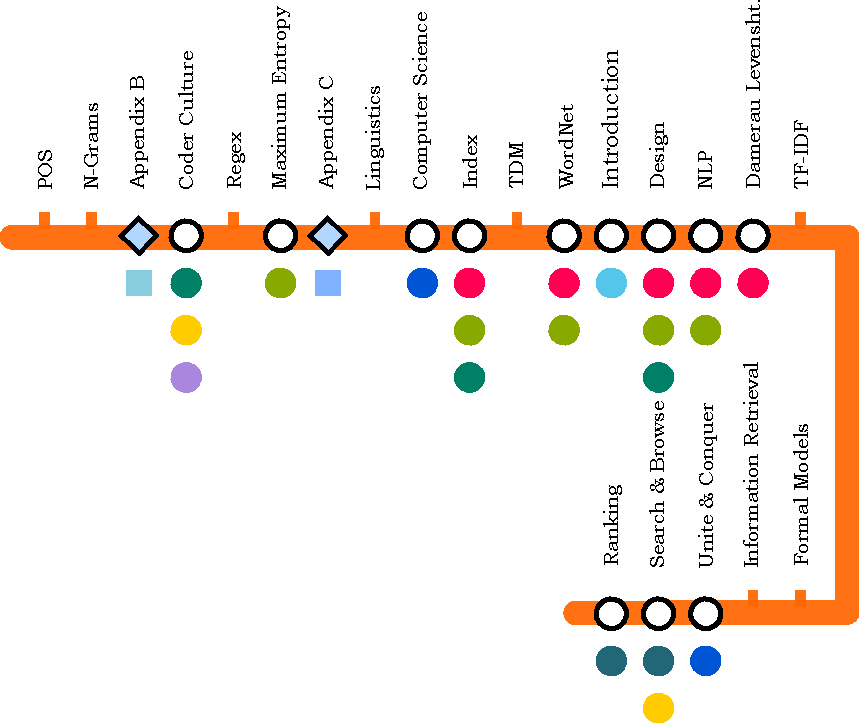
\includegraphics{tech.pdf}
\end{figure}

\vfill

{\sffamily 
Hello World \intro, test vlah blah dhfsdhf sdifh sohdsld hf sdfh h ghdls hg. Hello World \intro, whats up \inspi~ and helllo to you too \appa~ test,. ksjdfkj sdkjgh  ksdhg sdjfh sdjfh ksdfjhsdkfhskh kgh kjhfdg kjhgfhjfh sjueyuh tyb jjhg.
Hello World \intro, test vlah blah dhfsdhf sdifh sohdsld hf sdfh h ghdls hg. Hello World \intro, whats up \inspi~ and helllo to you too \appa~ test,. ksjdfkj sdkjgh  ksdhg sdjfh sdjfh ksdfjhsdkfhskh kgh kjhfdg kjhgfhjfh sjueyuh tyb jjhg.
Hello World \intro, test vlah blah dhfsdhf sdifh sohdsld hf sdfh h ghdls hg. Hello World \intro, whats up \inspi~ and helllo to you too \appa~ test,. ksjdfkj sdkjgh  ksdhg sdjfh sdjfh ksdfjhsdkfhskh kgh kjhfdg kjhgfhjfh sjueyuh tyb jjhg.
}

\begin{figure}[!htbp]
\centering
  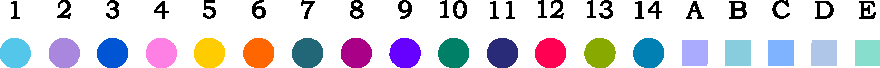
\includegraphics[width=\textwidth]{legend.pdf}
\end{figure}

\newpage
\minicontents
\spirals


\section{Information Retrieval}

\begin{quotation}
  Information retrieval deals with the representation, storage, organisation of, and access to information items such as documents, Web pages, online catalogs, structured and semi-structured records, multimedia objects. The representation and organisation of the information items should be such as to provide the users with easy access to information of their interest. \sourceatright{\autocite{Baeza-Yates2011}}
\end{quotation}

In simple terms, a typical search process can be described as follows (see figure~\ref{fig:sea}\marginpar{\faicon{object-group}~\ref{fig:sea}}). A user is looking for some information so she or he types a search term or a question into the text box of a search engine. The system analyses this query and retrieves any matches from the index, which is kept up to date by a web crawler. A ranking algorithm then decides in what order to return the matching results and displays them for the user. In reality of course this process involves many more steps and level of detail, but it provides a sufficient enough overview.

\begin{figure}[!htbp]
  \centering
  \begin{tikzpicture}[node distance = 1cm and 2cm]
    \node [box] (web) {Web};
    \node [box, below = of web] (crawl) {Crawler};
    \node [box, below = of crawl] (index) {Index};
    \node [box, right = of web] (user) {User};
    \node [box, below = of user] (query) {Query};
    \node [box, below = of query] (rank) {Ranking};
    \draw [sa] (web) -- (crawl);
    \draw [sa] (crawl) -- (index);
    \draw [sa] (user) -- (query);
    \draw [sa] (index) -- (rank);
    \draw [sa] (rank) -| +(1.4,0) |- (user);
    \draw [sa] (query.west) -| +(-1,0) |- (index.north east);
  \end{tikzpicture}
\caption[Search engine architecture]{Abstract search engine architecture}
\label{fig:sea}
\end{figure}

Most big web search engines like Google, Baidu or Bing focus on usefulness and relevance of their results \autocite{Google2012, Baidu2012, Microsoft2012a}. Google uses over 200 signals \autocite*{Google2012} that influence the ranking of web pages including their original PageRank algorithm \autocite{Brin1998, Brin1998b}.

Any \ac{IR} process is constrained by factors like subject, context, time, cost, system and user knowledge \autocite{Marchionini1988}. Such constraints should be taken into consideration in the development of any search tool. A web crawler needs resources to crawl around the web, language barriers may exist, the body of knowledge might not be suitable for all queries, the system might not be able to cater for all types of queries (e.g.\ single-word vs.\ multi-word queries), or the user might not be able to understand the user interface, and many more. It is therefore imperative to eliminate certain constraining factors---for example by choosing a specific target audience or filtering the amount of information gathered by a crawler from web pages.

The crawler, sometimes called spider, indexer or bot, is a program that processes and archives information about every available webpage it can find. It does this by looking at given `seed' pages and searching them for hyperlinks. It then follows all of these links and repeats the process over and over. The Googlebot \autocite*{Google2016} and the Bingbot \autocite*{Bing2016} are well-known examples.

An index is a list of keywords (called the dictionary or vocabulary) together with a list called `postings list' that indicates the documents in which the terms occur. One way to practically implement this is to create a \ac{TDM} as shown in equation~\ref{eq:tdm}\marginpar{$\bm{\Sigma}$~\ref{eq:tdm}}.

\begin{equation}
  \bbordermatrix{~ & d_1 & d_2 \cr
        k_1 & f_{1,1} & f_{1,2} \cr
        k_2 & f_{2,1} & f_{2,2} \cr
        k_3 & f_{3,1} & f_{3,2}}
\label{eq:tdm}
\end{equation}
% \myequations{Term-document matrix}

where $f_{i,j}$ is the frequency of term $k_{i}$ in document $d_{j}$. To illustrate this with a concrete example, figure~\ref{fig:termdocs}\marginpar{\faicon{object-group}~\ref{fig:termdocs}} shows a \ac{TDM} for a selection of words in a corpus containing three documents\footnote{These texts are part of one of the two corpora used for \url{pata.physics.wtf}. More information about this can be found in chapters~\ref{s:faustlib} and ~\ref{s:corpora}.}.

\begin{itemize}
  \item Alfred Jarry: \textit{Exploits and Opinions of Dr.\ Faustroll, $'$Pataphysician} (`Faustroll') \autocite*{Jarry1996}
  \item Saint Luke: \textit{The Gospel} (`Gospel') \autocite*{Luke2005}
  \item Jules Verne: \textit{A Journey to the Centre of the Earth} (`Voyage') \autocite*{Verne2010}
\end{itemize}

\begin{figure}[!htbp]
\[
  \bbordermatrix{
    ~                  & \text{Faustroll} & \text{Gospel} & \text{Voyage} \cr
    \text{Faustroll}   & 77               & 0             & 0             \cr
    \text{father}      & 1                & 28            & 2             \cr
    \text{time}        & 34               & 16            & 129           \cr
    \text{background}  & 0                & 0             & 0             \cr
    \text{water}       & 29               & 7             & 120           \cr
    \text{doctor}      & 30               & 0             & 0             \cr
    \text{without}     & 27               & 7             & 117           \cr
    \text{bishop}      & 27               & 0             & 2             \cr
    \text{God}         & 25               & 123           & 2
  }
\]
\caption[Example TDM]{Example TDM for 3 documents and 9 words}
\label{fig:termdocs}
\end{figure}

% purpose     & 2         & 0       & 3       \cr
% little      & 28        & 16      & 81      \cr
% skiff       & 35        & 0       & 0       \cr
% substance   & 8         & 3       & 1       \cr
% issue       & 0         & 2       & 2       \cr
% watch       & 5         & 3       & 6

% The total wordcount of the above files is as follows: Faustroll=\num{131891}, Gospel=\num{139669}, and Voyage=\num{497295}.

The dictionary is usually pre-processed (see section~\ref{s:nlp})\marginpar{§~\ref{s:nlp}} to eliminate punctuation and so-called `stop-words'\footnote{A full list of stopwords in English, French and German can be found in appendix~\ref{s:stopwords}.}\marginpar{§~\ref{s:stopwords}} (e.g. I, a, and, be, by, for, the, on, etc.) which would be useless in everyday text search engines. For specific domains it even makes sense to build a `controlled vocabulary', where only very specific terms are included (for example the index at the back of a book). This can be seen as a domain specific taxonomy and is very useful for query expansion (explained in the next paragraph).

Relevance feedback is an idea of improving the search results by explicit or implicit methods. Explicit feedback asks users to rate results according to their perceived relevance or collects that kind of information through analysis of mouse clicks, eye tracking, etc. Implicit feedback occurs when external sources are consulted such as thesauri or by analysing the top results provided by a search engine. There are two ways of using this feedback. It can be displayed as a list of suggested search terms to the user and the user decides whether or not to take the advice, or the query is modified internally without the user's knowledge. This is then called automatic query expansion.


\subsection{IR Models}
\label{s:irmodels}

There are different models for different needs, for example a multimedia system is going to be different than a text based \ac{IR} system, and a web based system is going to be different than an offline database system. Even within one such category there could more than one model. Take text based search systems for example. Text can be unstructured or semi-structured. Web pages are typically semi-structured. They contain a title, different sections and paragraphs and so on. An unstructured page would have no such differentiations but only contain simple text.  Classic example models are set-theoretic, algebraic and probabilistic. The PageRank algorithm by Google is a link-based retrieval model \autocite{Brin1998}.

The notation for \ac{IR} models is a quadruple $[D,Q,F,R(q_i, d_j)]$ \autocite[adapted from][]{Baeza-Yates2011} where,

\begin{conditions}
  D           & the set of documents \\
  Q           & the set of queries \\
  F           & the framework e.g.\ sets, Boolean relations, vectors, linear algebra\ldots \\
  R(q_i, d_j) & the ranking function, with $q_i \in Q$ and $d_j \in D$ \\
  t           & the number of index terms in a document collection \\
  V           & the set of all distinct index terms $\{k_1,\ldots, k_t\}$ in a document collection (vocabulary)
\end{conditions}

This means, given a query $q$ and a set of documents $D$, we need to produce a ranking score $R(q, d_j)$ for each document $d_j$ in $D$.


\subsubsection{The Boolean Model}

One such ranking score is the Boolean model. The similarity of document $d_j$ to query $q$ is defined as follows \autocite{Baeza-Yates2011}

\begin{equation}
  sim(d_j,q) =
  \begin{cases}
  1 & \text{if} \ \exists \ c(q) \ | \ c(q) = c(d_j)\\
  0 & \text{otherwise}
  \end{cases}
  \label{eq:sim}
\end{equation}
% \myequations{sim}

where $c(x)$ is a `conjunctive component' of $x$. A conjunctive component is one part of a declaration in \ac{DNF}. It describes which terms occur in a document and which ones do not. For example, for vocabulary $V =\{k_0,k_1,k_2\}$, if all terms occur in document $d_j$ then the conjunctive component would be $(1,1,1)$, or $(0,1,0)$ if only term $k_1$ appears in $d_j$. Let's make this clearer with a practical example. Figure~\ref{fig:termdocs2}\marginpar{\faicon{object-group}~\ref{fig:termdocs2}} (a shorter version of figure~\ref{fig:termdocs}) shows a vocabulary of 4 terms over 3 documents. 

\begin{figure}[!htbp]
\[
  \bbordermatrix{
    ~                  & \text{Faustroll} & \text{Gospel} & \text{Voyage} \cr
    \text{Faustroll}   & 77               & 0             & 0             \cr
    \text{time}        & 34               & 16            & 129           \cr
    \text{doctor}      & 30               & 0             & 0             \cr
    \text{God}         & 25               & 123           & 2
  }
\]
\caption[Example TDM (short)]{Example TDM for 9 words and 3 documents (short)}
\label{fig:termdocs2}
\end{figure}

So, we have a vocabulary $V$ of \{Faustroll, time, doctor and God\} and three documents $d_0 =$ Faustroll, $d_1 =$ Gospel and $d_2 =$ Voyage. The conjunctive component for $d_0$ is $(1,1,1,1)$. This is because each term in $V$ occurs at least once. $c(d_1)$ and $c(d_2)$ are both $(0,1,0,1)$ since the terms `Faustroll' and `doctor' do not occur in either of them.

Assume we have a query $q =$ doctor $\land$ (Faustroll $\lor$ $\neg$ God). Translating this query into \ac{DNF} will result in the following expression: $q_{DNF} = (1,0,1,1) \lor (1,1,1,1) \lor (1,0,1,0) \lor (1,1,1,0) \lor (0,0,1,0) \lor (0,1,1,0)$, where each component $(x_0,x_1,x_2,x_3)$ is the same as $(x_0 \land x_1 \land x_2 \land x_3)$.

% (1,0,1,1) F,D,G
% (1,1,1,1) F,T,D,G
% (1,0,1,0) F,D
% (1,1,1,0) F,T,D
% (0,0,1,0) D
% (0,1,1,0) T,D

One of the conjunctive components in $q_{DNF}$ must match a document conjunctive component in order to return a positive result. In this case $c(d_0)$ matches the second component in $q_{DNF}$ and therefore the Faustroll document matches the query $q$ but the other two documents do not.

The Boolean model gives `Boolean' results. This means something is either true or false. Sometimes things are not quite black and white though and we need to weigh the importance of words somehow.


\subsubsection{TF-IDF}
\label{s:tfidf}

One simple method of assigning a weight to terms is the so-called \acl{TF}-\acl{IDF} or \acs{TF}-\acs{IDF} for short. Given a \acs{TF} of $tf_{i,j}$ and a \acs{IDF} of $idf_i$ it is defined as $tf_{i,j}\times idf_i$ \autocite{Baeza-Yates2011}.

The \ac{TF} $tf_{i,j}$ is calculated and normalised using a log function as:
$1+\log_2 f_{i,j} \ \text{if} \ f_{i,j} > 0 \ \text{or} \ 0 \ \text{otherwise}$ where $f_{i,j}$ is the frequency of term $k_i$ in document $d_j$.

The \ac{IDF} $idf_i$ weight is calculated as $\log_2 (N/df_i)$, where the document frequency $df_i$ is the number of documents in a collection that contain a term $k_i$ and $idf_i$ is the \ac{IDF} of term $k_i$. The more often a term occurs in different documents the lower the \ac{IDF}. $N$ is the total number of documents.

\begin{equation}
  tfidf_{i,j} =
  \begin{cases}
  (1+\log_2 f_{i,j})\times \log_2\frac{N}{df_i} & \text{if} \ f_{i,j} > 0 \\
  0 & \text{otherwise}
  \end{cases}
  \label{eq:tfidfij}
\end{equation}
% \myequations{TF-IDF Ranking}

where $tfidf_{i,j}$ is the weight associated with $(k_i,d_j)$. Using this formula ensures that rare terms have a higher weight and more so if they occur a lot in one document. Table~\ref{tab:tfidf}\marginpar{\faicon{table}~\ref{tab:tfidf}} shows the following details.

\begin{conditions}
  k_{0}-k_{8} & [Faustroll,father,time,background,water,doctor,without,bishop,God] \\
  d_{0}-d_{2} & [Faustroll, Gospel, Voyage] (see figure~\ref{fig:termdocs}) \\
  f_{i,j}     & the frequence (count) of term $k_i$ in document $d_j$\\
  tf_{i,j}    & the \acl{TF} weight \\
  idf_{i}     & the \acl{IDF} weight \\
  tfidf_{i,j} & the \ac{TF}-\ac{IDF} weight
\end{conditions}

\begin{table}[!htbp]
\centering\small
\caption[TF-IDF weights]{\ac{TF}-\ac{IDF} weights}
\label{tab:tfidf}
\begin{tabu}{lllllllllllllll}
\toprule
& & & & \multicolumn{3}{c}{$\bm{d_0}$} & & \multicolumn{3}{c}{$\bm{d_1}$} & & \multicolumn{3}{c}{$\bm{d_2}$} \\
\cmidrule{5-7}\cmidrule{9-11}\cmidrule{13-15}
& & $idf$ & & $f$ & $tf$ & $tfidf$ & & $f$ & $tf$ & $tfidf$ & & $f$ & $tf$ & $tfidf$ \\
\midrule
$\bm{k_0}$ & & 1.58 & & 77 & 7.27 & 11.49 & & 0 & 0 & 0 & & 0 & 0 & 0 \\
$\bm{k_1}$ & & 0 & & 1 & 1 & 0 & & 28 & 5.81 & 0 & & 2 & 2 & 0 \\
$\bm{k_2}$ & & 0 & & 34 & 6.09 & 0 & & 16 & 5 & 0 & & 129 & 8.01 & 0 \\
$\bm{k_3}$ & & 0 & & 0 & 0 & 0 & & 0 & 0 & 0 & & 0 & 0 & 0 \\
$\bm{k_4}$ & & 0 & & 29 & 5.86 & 0 & & 7 & 3.81 & 0 & & 120 & 7.91 & 0 \\
$\bm{k_5}$ & & 1.58 & & 30 & 5.91 & 9.34 & & 0 & 0 & 0 & & 0 & 0 & 0 \\
$\bm{k_6}$ & & 0 & & 27 & 5.75 & 0 & & 7 & 3.81 & 0 & & 117 & 7.87 & 0 \\
$\bm{k_7}$ & & 0.58 & & 27 & 5.75 & 3.34 & & 0 & 0 & 0 & & 2 & 2 & 1.16 \\
$\bm{k_8}$ & & 0 & & 25 & 5.64 & 0 & & 123 & 7.94 & 0 & & 2 & 2 & 0 \\ 
\bottomrule
\end{tabu}
\end{table}

What stands out in table~\ref{tab:tfidf}\marginpar{\faicon{table}~\ref{tab:tfidf}} is that the $tfidf_{i,j}$ function returns \num{0} quite often. This is partially due to the $idf_i$ algorithm returning \num{0} when a term appears in all documents in the corpus. In the given example this is the case a lot but in a real-world example it might not occur as much.


\subsubsection{The Vector Model}

The vector model allows more flexible scoring since it basically computes the `degree' of similarity between a document and a query \autocite{Baeza-Yates2011}. Each document $d_j$ in the corpus is represented by a document vector $\vec{d_j}$ in $t$-dimensional space, where $t$ is the total number of terms in the vocabulary. Figure~\ref{fig:docvect}\marginpar{\faicon{object-group}~\ref{fig:docvect}} gives an example of vector $\vec{d_j}$ for document $d_j$ in 3-dimensional space. That is, the vocabulary of this system consists of three terms $k_a$, $k_b$ and $k_c$. A similar vector $\vec{q}$ can be constructed for query $q$. Figure~\ref{fig:VM}\marginpar{\faicon{object-group}~\ref{fig:VM}} then shows the similarity between the document and the query vector as the cosine of $\theta$.

\begin{figure}[!htbp] % (here, top, bottom, page)
  \centering
  \begin{minipage}[t]{.45\linewidth}
    \tdplotsetmaincoords{60}{120} %xz
    \begin{tikzpicture} [tdplot_main_coords, 
    axis/.style={->}, 
    vector/.style={-stealth,thick}, 
    vector guide/.style={dashed,gray}]
    %standard tikz coordinate definition using x, y, z coords
    \coordinate (O) at (0,0,0);
    %tikz-3dplot coordinate definition using x, y, z coords
    \pgfmathsetmacro{\ax}{2.5}
    \pgfmathsetmacro{\ay}{2.5}
    \pgfmathsetmacro{\az}{2.5}
    \coordinate (P) at (\ax,\ay,\az);
    %draw axes
    \draw[axis] (0,0,0) -- (3,0,0) node[anchor=north east]{$k_a$};
    \draw[axis] (0,0,0) -- (0,3,0) node[anchor=north west]{$k_b$};
    \draw[axis] (0,0,0) -- (0,0,3) node[anchor=south]{$k_c$};
    %draw a vector from O to P
    \draw[vector] (O) -- (P);
    %draw guide lines to components
    \draw[vector guide] (\ax,\ay,0) -- (P);
    \draw[vector guide]         (P) -- (0,0,\az);
    \draw[vector guide] (\ax,\ay,0) -- (0,\ay,0);
    \draw[vector guide] (\ax,\ay,0) -- (0,\ay,0);
    \draw[vector guide] (\ax,\ay,0) -- (\ax,0,0);
    %label vector
    \node[tdplot_main_coords,anchor=west]
    at (P){$\vec{d_j}$};
    \end{tikzpicture}
    \caption[A document vector]{A document vector $\vec{d_j}$}
    \label{fig:docvect}
  \end{minipage}
  \hspace{.05\linewidth}
  \begin{minipage}[t]{.45\linewidth}
    \begin{tikzpicture}
    \draw[->] (0,0) -- (3,0) coordinate (a) node[right] {$q$};
    \draw[->] (0,0) -- (2,2) coordinate (c) node[above right] {$d_j$};
    \draw (0,0) coordinate (b) node[left] {};
    \draw pic["$\theta$", draw=black, angle eccentricity=1.2, angle radius=1cm]
    {angle=a--b--c};
    \end{tikzpicture}
    \caption[The vector model]{The vector model}
    \label{fig:VM}
  \end{minipage}
\end{figure}

$\vec{d_j}$ is defined as $(w_{1,j}, w_{2,j}, \ldots, w_{t,j})$ and similarly $\vec{q}$ is defined as $(w_{1,q}, w_{2,q}, \ldots, w_{t,q})$, where $w_{i,j}$ and $w_{i,q}$ correspond to the \ac{TF}-\ac{IDF} weights per term of the relevant document or query respectively. $t$ is the total number of terms in the vocabulary. The similarity between a document $d_j$ and a query $q$ is defined in equation~\ref{eq:sim2}\marginpar{$\bm{\Sigma}$~\ref{eq:sim2}}.

\begin{equation}
  \begin{split}
  sim(d_j,q) &= \frac{\vec{d_j} \ \cdot \ \vec{q}}{|\vec{d_j}| \times |\vec{q}|}\\
  &= \frac{\sum_{i=1}^{t}w_{i,j} \times w_{i,q}}
  {\sqrt{\sum_{i=1}^{t}w_{i,j}^{2}} \times \sqrt{\sum_{i=1}^{t}w_{i,q}^{2}}}
  \end{split}
  \label{eq:sim2}
\end{equation}
% \myequations{sim2}

Let's consider an example similar to the one used for the \nameref{s:tfidf} section. We have a corpus of three documents ($d_0$ = Faustroll, $d_1$ = Gospel, and $d_2$ = Voyage) and nine terms in the vocabulary ($[k_0, \ldots, k_8]$ = (Faustroll, father, time, background, water, doctor, without, bishop, God)). The document vectors and their corresponding length is given below (with the relevant \ac{TF}-\ac{IDF} weights taken from table~\ref{tab:tfidf}\marginpar{\faicon{table}~\ref{tab:tfidf}}).

\begin{conditions}
  \vec{d_0}   & (11.49,0,0,0,0,9.34,0,3.34,0) \\
  |\vec{d_0}| & 15.18 \\
  \vec{d_1}   & (0,0,0,0,0,0,0,0,0) \\
  |\vec{d_1}| & 0 \\
  \vec{d_2}   & (0,0,0,0,0,0,0,1.16,0) \\
  |\vec{d_2}| & 1.16
\end{conditions}

For this example we will use two queries: $q_0$ (doctor, Faustroll) and $q_1$ (without, bishop). We then compute the similarity score for between each of the documents compared to the two queries by applying equation~\ref{eq:sim2}\marginpar{$\bm{\Sigma}$~\ref{eq:sim2}}. For the query $q_0$ the result clearly points to the first document, i.e. the Faustroll text. For query $q_1$ the score produces two results, with Verne's `Voyage' scoring highest.

\begin{figure}[!htbp] % (here, top, bottom, page)
  \centering
  \begin{minipage}[t]{.475\linewidth}
    \begin{conditions}
      q_0          & (doctor, Faustroll) \\
      \vec{q_0}    & (1.58,0,0,0,0,1.58,0,0,0) \\
      |\vec{q_0}|  & 2.24 \\
      sim(d_0,q_0) & 0.97 \\
      % 18.15 + 0 + 0 + 0 + 0 + 14.76 + 0 + 0 + 0 = 32.91
      % 15.18 * 2.24 = 34.00
      % 32.91 / 34 = 0.97
      sim(d_1,q_0) & 0 \\
      % 0 + 0 + 0 + 0 + 0 + 0 + 0 + 0 + 0 = 0
      % 0 * 2.24 = 0
      % 0 / 0 = 0
      sim(d_2,q_0) & 0
      % 0 + 0 + 0 + 0 + 0 + 0 + 0 + 0 + 0 = 0
      % 1.16 * 2.24 = 2.60
      % 0 / 2.60 = 0
    \end{conditions}
  \end{minipage}
  \hspace{.05\linewidth}
  \begin{minipage}[t]{.45\linewidth}
    \begin{conditions}
      q_1          & (without, bishop) \\
      \vec{q_1}    & (0,0,0,0,0,0,0,0.58,0) \\
      |\vec{q_1}|  & 0.58 \\
      sim(d_0,q_1) & 0.22 \\
      % 0 + 0 + 0 + 0 + 0 + 0 + 0 + 1.94 + 0 = 1.94
      % 15.18 * 0.58 = 8.80
      % 1.94 / 8.80 = 0.22
      sim(d_1,q_1) & 0 \\
      % 0 + 0 + 0 + 0 + 0 + 0 + 0 + 0 + 0 = 0
      % 0 * 0.58 = 0
      % 0 / 0 = 0
      sim(d_2,q_1) & 1
      % 0 + 0 + 0 + 0 + 0 + 0 + 0 + 0.67 + 0 = 0.67
      % 1.16 * 0.58 = 0.67
      % 0.67 / 0.67 = 1
    \end{conditions}
  \end{minipage}
\end{figure}

\spirals

There are several other common \ac{IR} models that aren't covered in detail here. These include the probabilistic, set-based, extended Boolean and fuzzy set {\sloppy \autocite{Miyamoto2010, Miyamoto1988, Srinivasan2001, Widyantoro2001, Miyamoto1986}} models or latent semantic indexing \autocite{Deerwester1990}, neural network models and others \autocite{Macdonald2009, Schuetze1998, Schuetze1995}.


\subsection{Searching vs. Browsing}
\label{s:browsing}

What is actually meant by the word `searching'? Usually it implies that there is something to be found, an \ac{IN}; although that doesn't necessarily mean that the searcher knows what he or she is looking for or how to conduct the search and satisfy that need.

From the user's point of view the search process can be broken down into four activities \autocite{Sutcliffe1998} reminiscent of classic problem solving techniques (mentioned briefly in chapter~\ref{s:4stages})\marginpar{§~\ref{s:4stages}} \autocite{Polya1957}:

\begin{description}[leftmargin=5cm]
  \item [Problem identification] \acf{IN},
  \item [Need articulation] \ac{IN} in natural language terms,
  \item [Query formulation] translate \ac{IN} into query terms, and
  \item [Results evaluation] compare against \ac{IN}.
\end{description}

This model poses problems in situations where an \ac{IN} cannot easily be articulated or in fact is not existent and the user is not looking for anything specific. This is not the only constraining factor though and Marchionini and Shneiderman have pointed out that ``the setting within which information-seeking takes place constrains the search process'' \autocite*{Marchionini1988} and they laid out a framework with the following main elements.

\begin{itemize}
  \item Setting (the context of the search and external factors such as time, cost)
  \item Task domain (the body of knowledge, the subject)
  \item Search system (the database or web search engine)
  \item User (the user’s experience)
  \item Outcomes (the assessment of the results/answers)
\end{itemize}

\spirals

Searching can be thought of in two ways, `information lookup' (searching) and `exploratory search' (browsing) \autocite{DeVries1993, Marchionini2006}. A situation where an \ac{IN} cannot easily be articulated or is not existent (i.e. the user is not looking for anything specific) can be considered a typical case of exploratory search. The former can be understood as a type of simple question answering while the latter is a more general and broad knowledge acquisition process without a clear goal.

Current web search engines are tailored for information lookup. They do really well in answering simple factoid questions relating to numbers, dates or names (e.g.\ fact retrieval, navigation, transactions, verification) but not so well in providing answers to questions that are semantically vague or require a certain extend of interpretation or prediction (e.g.\ analysis, evaluation, forecasting, transformation).

With exploratory search, the user’s success in finding the right information depends a lot more on constraining factors and can sometimes benefit from a combination of information lookup and exploratory search \autocite{Marchionini2006}.

\begin{quotation}
  Much of the search time in learning search tasks is devoted to examining and comparing results and reformulating queries to discover the boundaries of meaning for key concepts. Learning search tasks are best suited to combinations of browsing and analytical strategies, with lookup searches embedded to get one into the correct neighbourhood for exploratory browsing. \sourceatright{\autocite{Marchionini2006}}
\end{quotation}

De Vries called this form of browsing an ``enlargement of the problem space'', where the problem space refers to the resources that possibly contain the answers/solutions to the \ac{IN} \autocite*{DeVries1993}. This is a somewhat similar idea to that of Boden's conceptual spaces which she called the ``territory of structural possibilities'' and exploration of that space ``exploratory creativity'' \autocite{Boden2003} (see section~\ref{s:boden}\marginpar{§~\ref{s:boden}}).

% All of these ideas, however, seem to be concerned with how users interact with a search system, rather than how the system acts itself. So we need to shift our perspective and think about how a search tool can be more supportive for exploratory search directly and by what means.


\subsection{Ranking}
\label{s:ranking}

Ranking signals, such as the weights produced by the \ac{TF}-\ac{IDF} algorithm in section~\ref{s:tfidf}\marginpar{§~\ref{s:tfidf}}, contribute to the improvement of the ranking process. These can be content signals or structural signals. Content signals are referring to anything that is concerned with the text and content of a page. This could be simple word counts or the format of text such as headings and font weights. The structural signals are more concerned about the linked structure of pages. They look at incoming and outgoing links on pages. There are also web usage signals that can contribute to ranking algorithms such as the click-stream. This also includes things like the Facebook `like' button or the Google+ `+1' button which could be seen as direct user relevance feedback as well.

Ranking algorithms are the essence of any web search engine and as such guarded with much secrecy. They decide which pages are listed highest in search results and if their ranking criteria were known publically, the potential for abuse (such as `Google bombing' \autocite{Nicole2010} for instance) would be much higher and search results would be less trustworthy. Despite the secrecy there are some algorithms like Google's PageRank algorithm that have been described and published in academic papers.


\subsubsection{Algorithms}

\textit{PageRank} was developed by Larry Page and Sergey Brin as part of their Google search engine \autocite*{Brin1998b, Brin1998}. PageRank is a link analysis algorithm, meaning it looks at the incoming and outgoing links on pages. It assigns a numerical weight to each document, where each link counts as a vote of support in a sense. PageRank is executed at indexing time, so the ranks are stored with each page directly in the index. Brin and Page define the PageRank algorithm as follows \autocite*{Brin1998b}\marginpar{$\bm{\Sigma}$~\ref{eq:PR}}.

\begin{equation}
  PR(A) =
  (1 - d) + d (\sum_{i=1}^{n} \frac{PR(T_i)}{C(T_i)})
  \label{eq:PR}
\end{equation}
% \myequations{PR}

\begin{conditions}
  A    & the page we want to rank and is pointed to by pages $T_1$ to $T_n$ \\
  n    & the total number of pages on the Web graph \\
  C(A) & the number of outgoing links of page $A$ \\
  d    & a `damping' parameter set by the system (typically 0.85) needed to deal with dead ends in the graph
\end{conditions}

Figure~\ref{fig:pagerank}\marginpar{\faicon{image}~\ref{fig:pagerank}} which shows how the PageRank algorithm works. Each smiley represents a webpage. The colours are of no consequence. The smile-intensity indicates a higher rank or score. The pointy hands are hyperlinks. The yellow smiley is the happiest since it has the most incoming links from different sources with only one outgoing link. The blue one is slightly smaller and slightly less smiley even though it has the same number of incoming links as the yellow one because it has more outgoing links. The little green faces barely smile since they have no incoming links at all.

\begin{figure}[!htbp] % (here, top, bottom, page)
  \centering
  \includegraphics[width=.75\linewidth]{pagerank}
\caption[PageRank algorithm]{PageRank algorithm illustration \autocite{Wikimedia2012}}
\label{fig:pagerank}
\end{figure}

The HITS algorithm also works on the links between pages \autocite{Kleinberg1999, Kleinberg1999a}. HITS stands for `Hyperlink Induced Topic Search' and its basic features are the use of so called hubs and authority pages. It is executed at query time. Pages that have many incoming links are called `authorities' and page with many outgoing links are called `hubs'. Equation~\ref{eq:HITS}\marginpar{$\bm{\Sigma}$~\ref{eq:HITS}} shows the algorithm \autocite{Baeza-Yates2011}, where $S$ is the set of pages, $H(p)$ is the hub value for page $p$, and $A(p)$ is the authority value for page $p$.

\begin{equation}
  \begin{split}
  H(p) &= \sum_{u\in S \mid p\to u}A(u)\\
  A(p) &= \sum_{v\in S \mid v\to p}H(v)
  \end{split}
  \label{eq:HITS}
\end{equation}
% \myequations{HITS}

Hilltop is a similar algorithm with the difference that it operates on a specific set of expert pages as a starting point. It was defined by Bharat and Mihaila \autocite*{Bharat2000}. The expert pages they refer to should have many outgoing links to non-affiliated pages on a specific topic. This set of expert pages needs to be pre-processed at the indexing stage. The authority pages they define must be linked to by one of their expert pages. The main difference to the HITS algorithm then is that their `hub' pages are predefined.

Another algorithm is the so called Fish search algorithm \autocite{DeBra1994, DeBra1994a, DeBra1994b}. The basic concept here is that the search starts with the search query and a seed \ac{URL} as a starting point. A list of pages is then built dynamically in order of relevance following from link to link. Each node in this directed graph is given a priority depending on whether it is judged to be relevant or not. \ac{URL}s with higher priority are inserted at the front of the list while others are inserted at the back. Special here is that the `ranking' is done dynamically at query time.

There are various algorithms that follow this approach. For example the shark search algorithm \autocite{Hersovici1998}. It improves the process of judging whether or not a given link is relevant or not. It uses a simple vector model with a fuzzy sort of relevance feedback. Another example is the improved fish search algorithm \autocite{Luo2005} where an extra parameter allows more control over the search range and time. The Fish School Search algorithm is another approach based on the same fish inspiration \autocite{BastosFilho2008}. It uses principles from genetic algorithms and particle swarm optimization. Another genetic approach is Webnaut \autocite{Nick2001}.

Other variations include the incorporation of user behaviour \autocite{Agichtein2006}, social annotations \autocite{Bao2007}, trust \autocite{Garcia-Molina2004}, query modifications \autocite{Glover2001}, topic sensitive PageRank \autocite{Haveliwala2003}, folksonomies \autocite{Hotho2006}, SimRank \autocite{Jeh2002}, neural-networks \autocite{Shu1999}, and semantic web \autocite{Widyantoro2001,Du2007,Ding2004,Kamps2010,Taye2009}.


\subsection{Challenges}

Other issues that arise when trying to search the \ac{WWW} were identified by Baeza-Yates and Ribeiro-Neto as follows \autocite*{Baeza-Yates2011}.

\begin{itemize}
  \item Data is distributed. Data is located on different computers all over the world and network traffic is not always reliable.
  \item Data is volatile. Data is deleted, changed or lost all the time so data is often out-of-date and links broken.
  \item The amount of data is massive and grows rapidly. Scaling of the search engine is an issue here.
  \item Data is often unstructured. There is no consistency of data structures.
  \item Data is of poor quality. There is no editor or censor on the Web. A lot of data is redundant too.
  \item Data is not heterogeneous. Different data types (text, images, sound, video) and different languages exist.
\end{itemize}

Since a single query for a popular word can results in millions of retrieved documents from the index, search engines usually adopt a lazy strategy, meaning that they only actually retrieve the first few pages of results and only compute the rest when needed \autocite{Baeza-Yates2011}. To handle the vast amounts of space needed to store the index, big search engines use a massive parallel and cluster-based architecture \autocite{Baeza-Yates2011}. Google for example uses over \num{15000} commodity-class PCs that are distributed over several data centres around the world \autocite{Dean2003}.


\section{Natural Language Processing}
\label{s:nlp}

\acf{NLP} is a discipline within computer science which is also known as follows \autocite{Jurafsky2009}.

\begin{itemize}
  \item Speech and language processing
  \item Human language technology
  \item Computational linguistics
  \item Speech recognition and synthesis
\end{itemize}

Goals of \ac{NLP} are to get computers to perform useful tasks involving human language such as enabling human-machine communication, improving human-human communication, and text and speech processing. Applications are for example machine translation, automatic speech recognition, natural language understanding, word sense disambiguation, spelling correction, and grammar checking.

There are many tools and libraries available for \ac{NLP}, including the \ac{NLTK} Python library \autocite{Bird2009, NLTK2016} and WordNet \autocite{Princeton2010} (both of which were used for \url{pata.physics.wtf}).


\subsection{Words}

A `lemma' is a set of lexical forms that have the same stem (e.g.\ go). A `word-form' is the full inflected or derived form of the word (e.g.\ goes). A `word type' is a distinct word in a corpus (repetitions are not counted but case sensitive). A `word token' is any word (repetitions are counted repeatedly). Manning et al. list the following activities related to the word processing of text \autocite*{Manning2009}.

\begin{description}
  \item [Tokenisation] discarding white spaces and punctuation and making every term a token
  \item [Normalisation] making sets of words with same meanings, e.g.\ car and automobile
  \item [Case-folding] converting everything to lower case
  \item [Stemming] removing word endings, e.g.\ connection, connecting, connected $\to$ connect
  \item [Lemmatisation] returning dictionary form of a word, e.g.\ went $\to$ go
\end{description}


\subsubsection{WordNet}
\label{s:wordnet}

WordNet is a large lexical database for English, containing \num{166000} word form and sense pairs, useful for computational linguistics and \ac{NLP} \autocite{Miller1995}. A synset is a set of synonyms to represent a specific word sense. It is the basic building block of WordNet's hierarchical structure of lexical relationships.

\begin{quotation}
  Nouns, verbs, adjectives and adverbs are grouped into sets of cognitive synonyms (synsets), each expressing a distinct concept. Synsets are interlinked by means of conceptual-semantic and lexical relations. \sourceatright{\autocite{Princeton2010}}
\end{quotation}

\begin{description}[leftmargin=2.75cm]
  \item [Synonymy] (same-name) a symmetric relation between word forms
  \item [Antonymy] (opposing-name) a symmetric relation between word forms
  \item [Hyponymy] (sub-name) a transitive relation between synsets
  \item [Hypernymy] (super-name) inverse of hyponymy
  \item [Meronymy] (part-name) complex semantic relation
  \item [Holonymy] (whole-name) inverse of meronymy
  \item [Troponymy] (manner-name) is for verbs what hyponymy is for nouns
\end{description}

Other relations not used by WordNet are homonymy (same spelling but different sound and meaning) and heteronymy (same sound but different spelling), homography (same sound and spelling) and heterography (different sound and spelling).

Appendix~\ref{app:wordnet}\marginpar{§~\ref{app:wordnet}} shows an example result produced by WordNet rendered for a web browser. 


\subsubsection{Regular Expressions}
\label{s:regex}

Regular expressions (often shortened to the term `regex') are used to search a corpus of texts for the occurrence of a specific string pattern\footnote{There is also a Regex Crossword puzzle \autocite{Michelsen2016}.}.

% Online tools such as \url{http://regexr.com/} or \url{https://regex101.com/} can help create a particular expression and test it. 

Table~\ref{tab:regex}\marginpar{\faicon{table}~\ref{tab:regex}} shows the most common commands needed to build a regular expression. For example, to find an email address in a piece of text the following regex can be used:

\begin{minted}{text}
([a-zA-Z0-9_\-\.]+)@([a-zA-Z0-9_\-\.]+)\.([a-zA-Z]{2,5})
\end{minted}

Most modern text editors support a form of search using regex and it is often used in \ac{NLP}.

\begin{table}[!htbp]
\centering
\caption[Regular expression syntax]{Regular expression syntax}
\label{tab:regex}
\begin{tabu}{ll}
\toprule
\textbf{Command}           & \textbf{Description}         \\ 
\midrule
.                          & any character except newline \\
\textbackslash w \textbackslash d \textbackslash s & word, digit, whitespace      \\
\textbackslash W \textbackslash D \textbackslash S & not word, digit, whitespace  \\
{[}abc{]}                  & any of a, b, or c            \\
{[}\textasciicircum abc{]} & not a, b, or c               \\
{[}a-g{]}                  & character between a \& g     \\
\textasciicircum abc\$     & start / end of the string    \\
a* a+ a?                   & 0 or more, 1 or more, 0 or 1 \\
a\{5\} a\{2,\}             & exactly five, two or more    \\
ab|cd                      & match ab or cd               \\ 
\bottomrule
\end{tabu}
\end{table}


\subsubsection{Damerau-Levenshtein}

The Damerau–Levenshtein distance\marginpar{$\bm{\Sigma}$~\ref{eq:DL}} between two strings $a$ and $b$ is given by $d_{a,b}(|a|,|b|)$ (see equation~\ref{eq:DL}) \autocite{WikipediaA, Damerau1964, Levenshtein1966}. The distance indicates the number of operations (insertion, deletion, substitution or transposition) it takes to change one string to the other. For example, the words `clear' and `clean' would have a distance of 1, as it takes on substitution of the letter `r' to `n' to change the word. A typical application would be spelling correction. 

\begin{equation}
  d_{a,b}(i,j)=\left\{\begin{matrix*}[l]
  \max(i,j) & \textrm{if}\min(i,j)=0\\
  \min\left\{\begin{matrix*}[l]
  d_{a,b}(i-1,j)+1\\
  d_{a,b}(i,j-1)+1\\
  d_{a,b}(i-1,j-1)+1_{a_i\neq b_j}\\
  d_{a,b}(i-2,j-2)+1
  \end{matrix*}\right. & \textrm{if}\ i,j > 1 \ \textrm{and}\ a_i = b_{j-1}\ \textrm{and}\ a_{i-1} = b_j\\
  \min\left\{\begin{matrix*}[l]
  d_{a,b}(i-1,j)+1\\
  d_{a,b}(i,j-1)+1\\
  d_{a,b}(i-1,j-1)+1_{a_i\neq b_j}
\end{matrix*}\right. & \textrm{otherwise.}
  \end{matrix*}\right.
  \label{eq:DL}
\end{equation}
% \myequations{DL}

$1_{(a_i \neq b_j)}$ is equal to $0$ when $a_i = b_j$ and equal to $1$ otherwise. 

\begin{itemize}
  \item $d_{a,b}(i-1,j) + 1$ corresponds to a deletion (from a to b)
  \item $d_{a,b}(i,j-1) + 1$ corresponds to an insertion (from a to b)
  \item $d_{a,b}(i-1,j-1) + 1_{(a_i \neq b_j)}$  corresponds to a match or mismatch, depending on whether the respective symbols are the same
  \item $d_{a,b}(i-2,j-2) + 1$  corresponds to a transposition between two successive symbols
\end{itemize}


\subsection{Sequences}


\subsubsection{N-Grams}
\label{s:ngrams}

We can do word prediction with probabilistic models called $N$-Grams. They predict the probability of the next word from the previous $N-1$ words \autocite{Jurafsky2009}. A 2-gram is usually called a `bigram' and a 3-gram a `trigram'.

A basic way to compute the probability of an N-gram is using a \ac{MLE} shown in equation~\ref{eq:mle}\marginpar{$\bm{\Sigma}$~\ref{eq:mle}} \autocite{Jurafsky2009} of a word $w_n$ given some history $w_{n-N+1}^{n-1}$ (i.e. the previous words in the sentence for example).

\begin{equation}
  P(w_n \mid w_{n-N+1}^{n-1}) = \frac{C(w_{n-N+1}^{n-1} w_n)}{C(w_{n-N+1}^{n-1})}
  \label{eq:mle}
\end{equation}
% \myequations{Probwn} 

For instance, if we want to check which of two words ``shining'' and ``cold'' has a higher probability of being the next word given a history of ``the sun is'', we would need to compute $P$(shining|the sun is) and $P$(cold|the sun is) and compare the results. To do this we would have to divide the number of times the sentence ``the sun is shining'' occurred in a training corpus by the number of times ``the sun is'' occurred and the same for the word ``cold''.

Counts ($C$) are normalised between 0 and 1. These probabilities are usually generated using a training corpus. These training sets are bound to have incomplete data and certain N-grams might be missed (which will result in a probability of 0). Smoothing techniques help combat this problem. 

One example is the so-called `Laplace' or `add-one smoothing', which basically just adds 1 to each count. See equation~\ref{eq:padd1}\marginpar{$\bm{\Sigma}$~\ref{eq:padd1}} \autocite{Jurafsky2009}. $V$ is the number of terms in the vocabulary.

\begin{equation}
  P_{Add-1}(w_i \mid w_{i-1}) = \frac{c(w_{i-1}, w_i) + 1}{c(w_{i-1}) + V}
  \label{eq:padd1}
\end{equation}
% \myequations{padd1}

Another example of smoothing is the so-called `Good Turing discounting'. It uses ``the count of things you've seen \textit{once} to help estimate the count of things you've \textit{never seen}'' \autocite[their emphasis]{Jurafsky2009}.

\spirals

To calculate the probability of a sequence of $n$ words ($P(w_1,w_2,\ldots,w_n)$ or $P(w_1^n)$ for short) we can use the chain rule of probability as shown in equation~\ref{eq:probw1n}\marginpar{$\bm{\Sigma}$~\ref{eq:probw1n}} \autocite{Jurafsky2009}.

\begin{equation}
  \begin{split}
  P(w_1^n) &= P(w_1)P(w_2 \mid w_1)P(w_3 \mid w_1^2 ) \ldots P(w_n \mid w_1^{n-1})\\
  &= \prod_{k=1}^{n}P(w_k \mid w_1^{k-1})
  \end{split}
  \label{eq:probw1n}
\end{equation}
% \myequations{Probw1n}

Instead of using the complete history of previous words when calculating the probability of the next term, usually only the immediate predecessor is used. This assumption that the probability of a word\marginpar{$\bm{\Sigma}$~\ref{eq:probw1n2}} depends only on the previous word (or $n$ words) is the called a Markov assumption (see equation~\ref{eq:probw1n2} \autocite{Jurafsky2009}).

\begin{equation}
  P(w_1^n) = \prod_{k=1}^{n}P(w_k \mid w_{k-1})
  \label{eq:probw1n2}
\end{equation}
% \myequations{Probw1n2}


\subsubsection{Part-of-Speech Tagging}
\label{s:pos}

\ac{POS} are lexical tags for describing the different elements of a sentence. The eight most well-known \ac{POS} are as follows.

\begin{description}[leftmargin=2.75cm]
  \item [Noun] an abstract or concrete entity
  \item [Pronoun] a substitute for a noun or noun phrase
  \item [Adjective] a qualifier of a noun
  \item [Verb] an action, occurrence, or state of being
  \item [Adverb] a qualifier of an adjective, verb, or other adverb
  \item [Preposition] an establisher of relation and context
  \item [Conjunction] a syntactic connector
  \item [Interjection] an emotional greeting or exclamation
\end{description}

More specialised sets of tags exist such as the \textit{Penn Treebank} tagset \autocite{Marcus1993} consisting of 48 different tags, including $CC$ for coordinating conjunction, $CD$ for cardinal number, $NN$ for noun singular, $NNS$ for noun plural, $NNP$ for proper noun singular, $VB$ for verb base form, $VBG$ for verb gerund, $DT$ for determiner, $JJ$ for adjectives, etc. A full table of these 48 tags can be found in appendix~\ref{s:penntreebank}\marginpar{§~\ref{s:penntreebank}}.

The process of adding tags to the words of a text is called `\ac{POS} tagging' or just `tagging'. Below, you can see an example tagged sentence\footnote{This is actually the very first sentence in Jarry's Faustroll book \autocite*{Jarry1996}.}.

\begin{quote}
  In\slash{}IN this\slash{}DT year\slash{}NN Eighteen\slash{}CD Hundred\slash{}CD and\slash{}CC Ninety-eight\slash{}CD,\slash{}, the\slash{}DT Eighth\slash{}CD day\slash{}NN of\slash{}IN February\slash{}NNP,\slash{}, Pursuant\slash{}JJ to\slash{}IN article\slash{}NN 819\slash{}CD of\slash{}IN the\slash{}DT Code\slash{}NN of\slash{}IN Civil\slash{}NNP Procedure\slash{}NNP and\slash{}CC at\slash{}IN the\slash{}DT request\slash{}NN of\slash{}IN M.\slash{}NN and\slash{}CC Mme.\slash{}NN Bonhomme\slash{}NNP (\slash{}(Jacques\slash{}NNP)\slash{}),\slash{}, proprietors\slash{}NNS of\slash{}IN a\slash{}DT house\slash{}NN situate\slash{}JJ at\slash{}IN Paris\slash{}NNP,\slash{}, 100\slash{}CD bis\slash{}NN,\slash{}, rue\slash{}NN Richer\slash{}NNP,\slash{}, the\slash{}DT aforementioned\slash{}JJ having\slash{}VBG address\slash{}NN for\slash{}IN service\slash{}NN at\slash{}IN my\slash{}PRP residence\slash{}NN and\slash{}CC further\slash{}JJ at\slash{}IN the\slash{}DT Town\slash{}NNP Hall\slash{}NNP of\slash{}IN Q\slash{}NNP borough\slash{}NN .\slash{}.
\end{quote}

% \begin{equation}
%   t_1^n = \underset{t_1^n}{\text{argmax}} \ P(w_1^n \mid t_1^n) P(t_1^n)
%   \label{eq:tn1}
% \end{equation}
% % \myequations{tn1}

% \begin{equation}
%   P(t_i \mid t_{i-1}) = \frac{C(t_{i-1},t_i)}{C(t_{i-1})}
%   \label{eq:pti}
% \end{equation}
% % \myequations{pti}

% For example: the probability of getting a common noun after a determiner is:

% \begin{equation}
%   P(\text{NN} \mid \text{DT}) = \frac{C(\text{DT},\text{NN})}{C(\text{DT})} = \frac{56,509}{116,454} = 0.49
%   \label{eq:pnndtt}
% \end{equation}
% % \myequations{pnndt}

% Given that there are $116,454$ occurrences of DT in the corpus and of these $56,509$ occurrences where a NN follows after the DT.% chktex 13

% \begin{equation}
%   P(\text{is} \mid \text{VBZ}) = \frac{C(\text{VBZ},\text{is})}{C(\text{VBZ})} = \frac{10,073}{21,627} = 0.47
%   \label{eq:pisvbz}
% \end{equation}
% % \myequations{pisvbz}

% Or the probability of a third person singular verb being `is' is 0.47.


\subsubsection{Maximum Entropy}
\label{s:maxent}

Hidden Markov or maximum entropy models can be used for sequence classification, e.g.\ part-of-speech tagging. 

\begin{quotation}
  The task of classification is to take a single observation, extract some useful features describing the observation, and then, based on these features, to classify the observation into one of a set of discrete classes. \sourceatright{\autocite{Jurafsky2009}}
\end{quotation}

A classifier like the maximum entropy model will usually produce a probability of an observation belonging to a specific class. Equation~\ref{eq:pcx}\marginpar{$\bm{\Sigma}$~\ref{eq:pcx}} shows how to calculate the probability of an obersvation (i.e. word) $x$ being of class $c$ as $p(c|x)$ \autocite{Jurafsky2009}.

\begin{equation}
  p(c|x) = \frac{\exp(\sum_{i=0}^{N}w_{ci}f_i(c,x))}{\sum_{c'\in C}\exp(\sum_{i=0}^{N}w_{c'i}f_i(c',x))}
  \label{eq:pcx}
\end{equation}
% \myequations{pcdlambda}

\begin{conditions}
f_i(c,x) & the feature (e.g. ``this word ends in \textit{-ing}'' or ``the previous word was \textit{the}'') \\
w_i      & the weight of the feature $f_i$
\end{conditions}

% \spirals

% This is best understood using an example from Jurafsky and Martin \autocite*{Jurafsky2009}.

% Consider the incompletely tagged sentence below. We want to find the most suitable tag for the word ``race''.

% \begin{quote}
%   Secretariat/NNP is/BEZ expected/VBN to/TO race/?? tomorrow/
% \end{quote}

% Features for $f_i(c,x)$ might have the following conditions. If these are true, the result would be 1, if false then 0.

% \begin{itemize}
%   \item $x= \text{``race'' } \& \ c = \text{NN}$
%   \item $t_{i-1}= \text{TO } \& \ c = \text{VB}$
%   \item $\text{suffix}(x)= \text{``ing'' } \& \ c = \text{VBG}$
%   \item $\text{is\_lower\_case}(x) \ \& \ c = \text{VB}$
%   \item $x = \text{``race''}\ \& \ c = \text{VB}$
%   \item $t_{i-1} = \text{TO}\ \& \ c = \text{NN}$
% \end{itemize}

% Weights are then assigned:

% \begin{table}[!htbp]
% \centering
% \caption{My caption}
% \label{tab:featweights}
% \begin{tabu}{llllllll}
% \toprule
%    &   & $\bm{f_1}$ & $\bm{f_2}$ & $\bm{f_3}$ & $\bm{f_4}$ & $\bm{f_5}$ & $\bm{f_6}$ \\
% \midrule
% \textbf{VB} & f & 0     & 1     & 0     & 1     & 1     & 0     \\
% \textbf{VB} & w &       & 0.8   &       & 0.01  & 0.1   &       \\
% \textbf{NN} & f & 1     & 0     & 0     & 0     & 0     & 1     \\
% \textbf{NN} & w &       & 0.8   &       &       &       & -1.3  \\
% \bottomrule
% \end{tabu}
% \end{table}


% To get the single best class with the highest probability we need to compute the following.

% \begin{equation}
%   \hat{c} = \underset{c\in C}{\text{argmax}} \ P(c \mid d,\lambda)
%   \label{eq:hatc}
% \end{equation}
% % \myequations{hatc}


% in quebec example
% \begin{table}[!htbp]
% \caption[MaxEnt Example table]{MaxEnt Example table}
% \label{tab:maxent}
%   \centering
%   \begin{tabu}{lll}
%   \toprule
%   PERSON    & LOCATION   & DRUG      \\ \midrule
%   In Québec & In Québec  & In Québec \\
%   0         & 1.8 + -0.6 & 0.3       \\
%   \bottomrule
%   \end{tabu}
% \end{table}

% Features:

% $f1(c,d) \equiv [ \ c = \text{LOCATION} \ \wedge \ w-1 = \text{``in''} \wedge \ \text{isCapitalized}(w)]$\\
% $f2(c,d) \equiv [ \ c = \text{LOCATION} \ \wedge \ \text{hasAccentedLatinChar}(w)]$\\
% $f3(c,d) \equiv [ \ c = \text{DRUG} \ \wedge \ \text{ends}(w,\text{``c''})]$

% $P(\text{LOCATION} \mid \text{in Québec}) = \frac{e^{1.8} e^{–0.6}}{e^{1.8} e^{–0.6} + e^{0.3} + e^0} = 0.586$\\
% $P(\text{DRUG} \mid \text{in Québec}) = \frac{e^{0.3}}{e^{1.8} e^{–0.6} + e^{0.3} + e^0} = 0.238$\\
% $P(\text{PERSON} \mid \text{in Québec}) = \frac{e^0}{e^{1.8} e^{–0.6} + e^{0.3} + e^0} = 0.176$


% The empirical expectation is the sum of all occurrences where a feature is true for one of our observed datums.

% \begin{equation}
%   empirical \ E(f_i)= \sum_{(c,d) \ \in \ observed(C,D)}f_i(c,d)
%   \label{eq:epirical}
% \end{equation}
% % \myequations{epirical}


\subsubsection{Grammars}
\label{s:grammars}

A language is modelled using a grammar, specifically a `Context-Free-Grammar'. Such a grammar normally consists or rules and a lexicon. For example a rule could be `NP $\to$ Det Noun', where NP stands for noun phrase, Det for determiner and Noun for a noun. The corresponding lexicon would then include facts like Det $\to$ a, Det $\to$ the, Noun $\to$ book. This grammar would let us form two noun phrases `the book' and `a book' only. Its two parse trees would then look like figure~\ref{fig:trees}\marginpar{\faicon{object-group}~\ref{fig:trees}}:

\begin{figure}[!htbp]
  \centering
  \begin{minipage}{.4\linewidth}
  \Tree[.NP [.Det \emph{a} ]
  [.Noun \emph{book} ]]
  \end{minipage}
  \hspace{.05\linewidth}
  \begin{minipage}{.4\linewidth}
  \Tree[.NP [.Det \emph{the} ]
  [.Noun \emph{book} ]]
  \end{minipage}
\caption[Parse trees]{Two parse trees for grammar `NP $\to$ Det Noun'}
\label{fig:trees}
\end{figure}

Parsing is the process of analysing a sentence and assigning a structure to it. Given a grammar, a parsing algorithm should produce a parse tree for a given sentence. The parse tree for the first sentence from Faustroll is shown below, in horizontal format for convenience. 

\begin{alltt}
(ROOT
  (S
    (PP (IN In)
      (NP (DT this) (NN year) (NNPS Eighteen) (NNP Hundred)
        (CC and)
        (NNP Ninety-eight)))
    (, ,)
    (NP
      (NP (DT the) (JJ Eighth) (NN day))
      (PP (IN of)
        (NP (NNP February) (, ,) (NNP Pursuant)))
      (PP
        (PP (TO to)
          (NP
            (NP (NN article) (CD 819))
            (PP (IN of)
              (NP
                (NP (DT the) (NNP Code))
                (PP (IN of)
                  (NP (NNP Civil) (NNP Procedure)))))))
        (CC and)
        (PP (IN at)
          (NP
            (NP (DT the) (NN request))
            (PP (IN of)
              (NP (NNP M.)
                (CC and)
                (NNP Mme) (NNP Bonhomme))))))
      (PRN (-LRB- -LRB-)
        (NP (NNP Jacques))
        (-RRB- -RRB-))
      (, ,)
      (NP
        (NP (NNS proprietors))
        (PP (IN of)
          (NP
            (NP (DT a) (NN house) (NN situate))
            (PP (IN at)
              (NP (NNP Paris))))))
      (, ,)
      (NP (CD 100) (NN bis))
      (, ,))
    (VP (VBP rue)
      (NP
        (NP (NNP Richer))
        (, ,)
        (NP (DT the) (JJ aforementioned)
          (UCP
            (S
              (VP (VBG having)
                (NP
                  (NP (NN address))
                  (PP (IN for)
                    (NP (NN service))))
                (PP (IN at)
                  (NP (PRP$ my) (NN residence)))))
            (CC and)
            (PP
              (ADVP (RBR further))
              (IN at)
              (NP
                (NP (DT the) (NNP Town) (NNP Hall))
                (PP (IN of)
                  (NP (NNP Q))))))
          (NN borough))))
    (. .)))
\end{alltt}

This particular tree was generated using the Stanford Parser \autocite*{Stanford2016}.


\subsubsection{Named Entity Recognition}

A named entity can be anything that can be referred to by a proper name, such as person, place or organisation names and times and amounts and these entities can be appropriately tagged.

Example (first sentence in Faustroll):

\begin{quote}
  In this [year Eighteen Hundred and Ninety-eight, the Eighth day of February]$^{\text{TIME}}$, Pursuant to article [819]$^{\text{NUMBER}}$ of the [Code of Civil Procedure]$^{\text{DOCUMENT}}$ and at the request of [M. and Mme. Bonhomme (Jacques)]$^{\text{PERSON}}$, proprietors of a house situate at [Paris, 100 bis, rue Richer]$^{\text{LOCATION}}$, the aforementioned having address for service at my residence and further at the [Town Hall]$^{\text{FACILITY}}$ of [Q borough]$^{\text{LOCATION}}$.
\end{quote}

So-called `gazetteers' (lists of place or person names for example) can help with the detection of these named entities.


\stopcontents[chapters]
